\begin{figure}
    \centering
    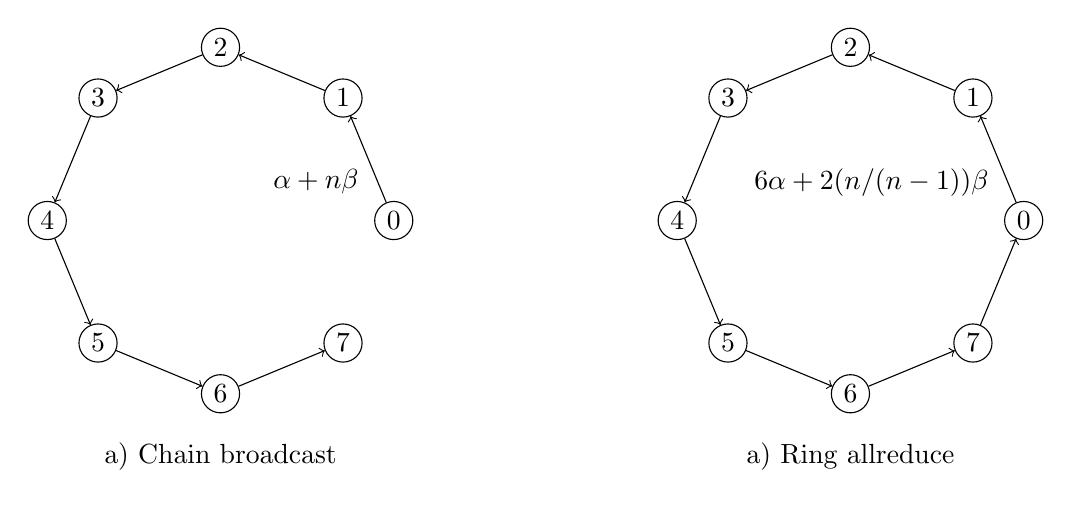
\begin{tikzpicture}[auto]
        \begin{scope}[shift={(4,0)}]
            \foreach \x in {0,1,...,7} {
                \node[circle,draw,inner sep=2pt] (A\x) at (\x*45:2.2) {\x} ;
            }
        \end{scope}
        
        \begin{scope}[shift={(-4,0)}]
            \foreach \x in {0,1,...,7} {
                \node[circle,draw,inner sep=2pt] (B\x) at (\x*45:2.2) {\x} ;
            }
        \end{scope}
        
        \node at (-4, -3) (Albl) {a) Chain broadcast};
        \node at (4, -3) (Blbl) {a) Ring allreduce};
        
        \path[->] (A0) edge[] node {$6\alpha+2(n/(n-1))\beta$} (A1)
                  (A1) edge[swap] node {} (A2)
                  (A2) edge[swap] node {} (A3)
                  (A3) edge node {} (A4)
                  (A4) edge node {} (A5)
                  (A5) edge[swap] node {} (A6)
                  (A6) edge[swap] node {} (A7)
                  (A7) edge[swap] node {} (A0);

        \path[->] (B0) edge node {$\alpha+n\beta$} (B1)
                  (B1) edge[swap] node {} (B2)
                  (B2) edge[swap] node {} (B3)
                  (B3) edge node {} (B4)
                  (B4) edge node {} (B5)
                  (B5) edge[swap] node {} (B6)
                  (B6) edge[swap] node {} (B7);

    \end{tikzpicture}
    \caption{
    Communication graphs for visualizing collective algorithms. 
    a) depicts a chain broadcast, while b) demonstrates a ring allreduce. 
    For both algorithms, all edge weights (represeting communication time) are the same, but the allreduce algorithm has to send more messages than the broadcast model.
    }
    \label{fig:graph-ring} 
\end{figure}